\documentclass[ notitlepage, numerical, 11pt]{revtex4-1} % style for Physical Review B and AJP are similar
\usepackage{float}
\usepackage{amsmath}

\usepackage{graphicx} 


\usepackage{sverb}

\begin{document}

\title{Physics of Non-Volatile Digital Data Storage Technologies}
\author{Tenzin Rigden}
\affiliation{Carleton College, Department of Physics, Northfield, MN 55057}
\date{\today}
\begin{abstract}
Data storage technologies have become increasingly important as more and more of our lives are being stored digitally in our phones and computers, and the need for higher density and faster data storage technologies increases. In this paper, I will talk about modern techniques such as optical disks, hard disk drives, and flash storage that are currently being used. In addition, I will talk about currently in development technologies such as holographic data storage and probe based storage that promises much higher densities than currently offered. 

\end{abstract}

\maketitle
\section{Introduction}
Computers and phones have become such a ubiquitous part of our lives that it is becoming more and more difficult to live without them. Just as important as these devices themselves are their contents. Your pictures, music, videos, papers, and more are all stored digitally on the devices. As more and more of our lives are recorded digitally, it has become increasingly important to find new ways to either expand our current data storage technologies or find new ones. On a fundamental level, a computer stores everything in a series of 1s or 0s called bits. In this binary system, 1 represents a ``true" state while a 0 represents a ``false" state. By using this binary system, it is possible to represent numbers as a sequence of 1s and 0s where each digit starting from the right represent an increasing power of 2 starting with $2^0$. For example, the number 13 can be represented as 1101 so we get, from the right, 1*$2^0$ + 0*$2^1$ + 1*$2^2$ + 1*$2^3$ which adds up to 13. Since we can represent numbers, we can use these numbers to represent other characters. One method is to use the American Standard Code for Information Interchange (ASCII) encoding system which was first published in 1963. ASCII encodes 128 characters that include letters, both lower case and capital, numbers, and other special characters into 7 bit integers. For example, the capital letter T corresponds to the 84th character and thus in binary can be represented as 01010100. A series of these binary numbers can be used to represent text.


Now that we know we can use binary to represent text, we can look at how we can physically store these 1s and 0s. One of the earlier methods was to use punch cards with holes and not holes representing 1s and 0s respectively. The early punch cards used 36 bits words because they were used in calculators and they wanted to be able to represent 10 decimal places. However this method is not very dense, data storage wise, and is limited by the number of holes that could be fit on a piece of paper.


In this paper, I will talk about more modern techniques that are currently being used for non-volatile memory, which means that data will not be lost if the device does not have power. I will begin with optical data storage, specifically optical disks. Then I will continue on to magnetic data storage specifcally talking about hard disk drives and their advancements. After that will be flash memory storage which promises much faster access to data. Lastly, I will talk about a state of the art technique currently being developed called holographic data storage which promises to greatly increase storage density.





\section{Optical Disk Storage}

Optical disks are a form of media storage that uses the grooves in the disk to store data. They have been commonplace in the United States since their invention in 1958 \cite{memory}. While optical disks aren't typically the preference by consumers for storing data directly from the computer, they are frequently used to archive or transfer data between machines. For optical disks, data is recorded and read using a laser beam. To record data onto a writable disc, a laser beam is shone on the reflective surface creating a pit, a tiny indentation, with a depth of the wavelength of the laser divided by 4. As seen in Fig. \ref{cdRom}, to read data, a very low power laser is shone on the disk and the reflected signal is converted to an electrical signal using a scanning photo detector. A binary value of 1 is recorded when there is a change in the surface depth due to switching to a pit to land or vice versa, and a 0 is interperted as when there is no change in the surface depth. When the laser is shone over an intersection between a pit and a land, there will be light reflected from the pit and the land resulting in two beams \cite{memory}. These two beams will then destructively interefere back at the photo-diode. To see how they interfere, we can look at it quantitatively. 

\begin{figure}[H]
\centerline{\includegraphics[scale=.9]{cdRom.png}}
\caption{ This is a cross-sectional view of a CD-ROM where there a pit signifies a $\lambda/4$ depth meaning when a laser shines over a change from land to pit or vice versa, destructive interference will take place signifying a bit value of 1$ http://www.hk-phy.org/articles/cdrom/cdrom_work_e.gif.$}
\label{cdRom}
\end{figure}

\subsection{Destructive Interference}
When two waves arrive at the same point the superpostion of those waves creates a new wave. Interference depends on the superposition of the waves and certain conditions. In our example, since we have a laser beam effectively being split into two beams, we have coherent light (there is a constant phase difference between two beams), and both beams have the same frequency. Then, we can define the electric field of the two beams as


\begin{align}
\begin{split}
\vec{E}_{1} = \vec{E}_{01} cos(k s_1-\omega t + \phi_1) \\
\vec{E}_{2} = \vec{E}_{02} cos(k s_1-\omega t + \phi_1),
\end{split}
\label{eRefInf}
\end{align}
where $ \vec{E}_{01}$ and $ \vec{E}_{02}$ are the amplitudes for the wave, $k$ is defined as $\frac{2\pi}{\lambda}$, $s_1$ and $s_2$ are defined as distance traveled by each beam, and $\phi_1$ and $\phi_2$ are the phases of the beams at t = 0 at their source \cite{optics}. Since we have the same source for both of our beams, the amplitudes and the phase at t = 0 are the same. Next, the superposition of these two waves at a point $P$ is 

\begin{equation}
\vec{E}_{P} = \vec{E}_{1} + \vec{E}_{2}.
\label{ePInf}
\end{equation}

The measurement of the effect of this wave on our eyes or a detector depends on the energy of the light beam. The irradiance, $I$, is the time average of the square of the wave amplitude and is is used to measure effects of waves \cite{optics}. The time average of the irradiance is done by the detector; our eye for example has an averaging time of 1/30 of a second. The irradiance is defined as 

\begin{equation}
I = \epsilon_0 c<\vec{E}_{P}\cdot \vec{E}_{P}>,
\label{iInf}
\end{equation}
where $\epsilon_0$ is the vacuum permittivity and $c$ is the speed of light \cite{optics}. By subbing in Eq. \ref{ePInf} for $\vec{E}_{P}$ and simplifying we get 
\begin{equation}
I = \epsilon_0 c<\vec{E}_{1}\cdot \vec{E}_{1}+\vec{E}_{2}\cdot \vec{E}_{2}+2\vec{E}_{1}\cdot \vec{E}_{2}>.
\label{iInf2}
\end{equation}
The first two terms correspond to the irradiances of the individual beams while the third term corresponds to the interaction between the waves and is the interference term, $I_{12}$ \cite{optics}. Then, $I$ can be rewritten as 
\begin{equation}
I = I_1 + I_2 + I_{12}.
\label{iInf3}
\end{equation}

The interference term, $I_{12}$, by using a trigonemtric identity and simplifying, can be written as 

\begin{equation}
I_{12} = 2\sqrt{I_1 I_2}<cos\delta>,
\label{iInf2}
\end{equation}
where $\delta$ is the phase difference and is defined as 
\begin{equation}
\delta = k(s_2 - s_1) +\phi_2 -\phi_1.
\label{delta}
\end{equation}
Finally, we can write $I$ as 
\begin{equation}
I = I_1 + I_2 +  2\sqrt{I_1 I_2}<cos\delta>.
\label{finalI}
\end{equation}
Destructive interference will yield a minimum value when $cos\delta$ is -1. In our case, since the beams have the same source, the laser, $\phi_1$ and $\phi_2$ are the same and their difference is 0, so $\delta$ will be 0 when the path length difference between the beams is $\frac{(2m+1)\lambda}{2}$ where m is an integer. Returning to our CD, since the pit has a depth of $\lambda/4$, the light reflected off of the pit will have a path length difference of $\lambda/2$ relative to the light reflected off of the land. This means that $\delta$ is $\pi$ so $cos\delta$ is -1. Since the sources for the beams are the same, $I_1$ = $I_2$, so our $I$ term is now
\begin{equation}
I = I_1 + I_1 - 2\sqrt{I_1 I_1} = 0.
\label{finalI2}
\end{equation}
This means at the change between a land and a pit, the two reflected beams will completely destructively interfere and no light will be reflected to the photo diode, which is then recorded as a 1. When there is no change in the surface depth, the light simply reflects back with no phase difference and is recorded as a 0 by the photo-diode \cite{memory}.

\subsection{Disk Types and Layers}
Optical Disks come in a few different styles: Compact Disk ROM (CD-ROM), CD-Recordable (CD-R), and Digital Versatile Disk (DVD). These disc technologies are written sequentially in a continous spiral track eminating from the middle out, the distance between each track is called the pitch. A CD-ROM is a disc that's only meant to be readable and is typically used for things such as installation of programs. Since it is only written once in the factory, a glass master disk is created using a high intensity laser. Liquid polycarbonate is inserted into the master disk to create a copy which is then covered with a reflective layer and then a protective layer over that. 
A CD-R is slightly different because it needs to be writable once outside of the factory. This is done by changing the structure of the disk to have a protective layer followed by a reflective layer, a painted layer, and a transparent layer as seen in Fig. \ref{cdR}. The painted layer is initially transparent and permantly becomes dark to simulate a pit when impacted by a high-intensity laser. This can then be read by a lower intensity laser that does not cause the painted layer to turn dark.



\begin{figure}[H]
\centerline{\includegraphics[scale=.45]{cdR.png}}
\caption{In this cross sectional view of a CD-R, the painted layer, if shone on by a high intensity laser will develop dark spots simulating pits \cite{memory}.}
\label{cdR}
\end{figure} 

\subsection{Rayleigh's Criteron due to Diffraction}

While CDs are useful and easy to carry around, their size was limited to only 700 MB until the early '90s when demand for higher storage capacities in the 1990s meant that the CD had to change. Since the 1 and 0 data values are stored in the pits and lands, the way to increase storage density was to decrease their size and also place tracks closer to each other by decreasing their pitch. However, these values can only be decreased to a certain point due to diffraction. Diffraction is the phenomenon where light that propagates through an opening interferes with itself causing a diffraction pattern. For lasers which use a circular aperture, the opening through which light travels, the diffraction pattern produced (as seen in Fig. \ref{airy}) is called an Airy Disk, with the bright circles representing maxima and the dark circles representing minima. This shape can be derived by starting with the electric field at point p through a circual aperture which can be found by 
\begin{equation}
E_p = \frac{E_A}{r_0}e^{i(k r_0 -\omega t)}\iint \limits_{Area} e^{i s k sin\theta} dA,
\label{EP}
\end{equation}
where $E_A$ is a constant factor that determines the strength of the electric field in the aperture, $k$ is the same as before $\frac{2\pi}{\lambda}$, $dA$ is an elemental area of the aperture as seen in Fig \ref{aperture}, $s$ is the radial distance from the center of the aperture to the $dA$, $\theta$ is the angle of the optical path relative to the axis orthogonal to the aperture, and $r_0$ is the optical path length to the point P \cite{optics}. 
\begin{figure}[H]
\centerline{\includegraphics[scale=.45]{bessel.jpg}}
\caption{\cite {optics.}}
\label{aperture}
\end{figure} 
We can write $dA$ as $xds$ where $x$ is $2\sqrt{R^2 - s^2}$ and $R$ is the aperture radius. Eq \ref{EP} then becomes 
\begin{equation}
E_p = 2\frac{E_A}{r_0}e^{i(k r_0 -\omega t)}\int_{-R}^R e^{i s k sin\theta}\sqrt{R^2 - s^2}ds.
\label{EP2}
\end{equation}
Next by making the following substitutions $v = \frac{s}{R}$ and $\gamma = kRsin\theta$, $E_P$ can be rewritten as
\begin{equation}
E_p = 2\frac{E_A R^2}{r_0}e^{i(k r_0 -\omega t)}\int_{-1}^1 e^{i \gamma v}\sqrt{1 - v^2}dv.
\label{EP3}
\end{equation}
The integral on the right side is known to be
\begin{equation}
\int_{-1}^1 e^{i \gamma v}\sqrt{1 - v^2}dv = \frac{\pi J_1(\gamma)}{\gamma},
\label{bessel}
\end{equation}
where $J_1(\gamma)$ is the first-order Bessel function of the first kind and can be represented by the infinite series \cite{optics}
\begin{equation}
J_1(\gamma) = \frac{\gamma}{2} - \frac{(\gamma /2)^3}{1^2 *2} + \frac{(\gamma /2)^5}{1^2 *2^2 *3} - .
\label{besselSeries}
\end{equation} 
Finally, the irradiance at point P can be written as 

\begin{equation}
I I_0(\frac{2J_1 (\gamma)}{\gamma})^2,
\label{iBessel}
\end{equation} 
where $\gamma = 1/2 k D sin\theta$, and $I_0$ is made up of all the other constants and is the irradiance at the principle maximum \cite{optics}. This function is what causes the light dark patterns in the Airy disk. In addition, the irradiance of the 2nd maximum as a ratio of $I_0$ is 0.0175. Because the principle maxiumum is so much larger than the 2nd, two point sources are considered resolvable when the principle maximum of one source overlaps with the first minimum of the other as in Fig. \ref{criterion} b. This is known as Rayleigh's Criterion. To create an equation for this criterion, we will need to know when the irradiance first becomes 0 and that distance from the center is the minimum resolvable distance. The irradiance first becomes 0 when $\gamma = 3.832$ so \cite{optics}
\begin{figure}[H]
\centerline{\includegraphics[scale=2]{220px-Airy-pattern.jpg}}
\caption{The airy disk created by a diffraction limited circular aperture lens laser \cite{airyDisk}.}
\label{airy}
\end{figure} 

\begin{equation}
\gamma = (\frac{k}{2})Dsin\theta = 3.832.
\label{gamma}
\end{equation}  
Using the small angle approximation and multiplying by the distance to the screen being projected onto, $f$, we get the minimum resolvable distance, d, as
\begin{equation}
d = f\frac{1.22\lambda}{D},
\label{minDF}
\end{equation}
$f$ is the focal length of the lens. Finally, $f/D$ can be re-written as $1/NA$ where $NA$ is the numerical aperture and indicates the resolving power of a lens. Subbing this into Eq. \ref{minDF}, we get Rayleigh's criterion \cite{memory}.
\begin{equation}
d = \frac{1.22\lambda}{2NA}.
\label{rayleigh}
\end{equation}
If all other optical instruments are perfect, this is the smallest resolvable distance from a laser. CDs use a laser wavelength of 780 nm along with a numerical aperture of .45 which yields a minimum resolvable distance of 1.06 microns. The actual resolvable distance for the laser in a CD isn't as perfect and is 1.6 microns. To decrease the minimum resolvable distance, and consequently decrease pit size and pitch, the numerical aperture must be increased and the wavelength of light decreased. This is what DVDs do.


\begin{figure}[H]
\centerline{\includegraphics[scale=.45]{criterion.png}}
\caption{The top image shows two resolable images, the middle image shows Rayleigh's critereon where the first fringe appears over the max of ther other image, and the bottom image shows them being not resolvable \cite{rayleigh}.}
\label{criterion}
\end{figure} 


DVDs use a laser of wavelength 650nm and numerical aperture of .6. This yields a real world minimum resolable distance of 1.1 microns and increases the storage density to 2.2GB/in$^2$ from 0.9Gb/in$^2$ of CDs \cite{memory}. Another innovation that allowed storage of up to 8.5GB was the ability to have two different recording layer: a semi reflective layer in the middle and a fully reflective layer at the other end. The different layers can be read by changing the focus of the laser. Additionally, instead of having a protective layer on one side of the disk, you can put another disc on it to effectively double the capacity again. However, this requires the manual flipping of the disc when accessing the other half of the data. By being double sided and having a double layer, DVDs can achieve a storage of 17GB \cite{memory}.

\begin{figure}[H]
\centerline{\includegraphics[scale=.45]{DVD.png}}
\caption{This is a cross section of a double sided and dual layer DVD. The pit and land information is stored at the two reflective and semi-reflective layers. The layer in which the laser is reading from is selected by focusing the laser to for that layer depth. To access the other side of the DVD, it must be physically removed and placed upside down \cite{memory}.}
\label{DVD}
\end{figure} 

A more recent innovation in storage of optical disks was the invention of the Blu-ray disc. Just like how using a smaller wavelength light in DVD compared to the ones in CD allowed the reduction in size of the pits and track size, Blu-ray discs also use a much shorter wavelength light to increase capacity. Blu-ray uses 405nm light which allows both the pit sizes and the track size, space between tracks, to be reduced to 0.15$\mu$m and 0.32$\mu$m respectively compared to the track size of 0.74$\mu$m for DVDs. This allows for a storage density of 14.7Gb/in$^2$ to be achieved \cite{memory}. 

\begin{figure}[H]
\centerline{\includegraphics[scale=.6]{cdPlay.png}}
\caption{This is the laser read system set up that corrects for depth errors with the positioning coil and corrects for reading off of the track error \cite{hyper}.}
\label{cdPlay}
\end{figure} 

\subsection{Laser Read System}

The implentation of the laser system used to read the data from the disk also worth looking into and can be seen in Fig. \ref{cdPlay}. The first part of this system from the source laser is the grating. The grating creates extra beams known as tracking beams, one on each side of the center beam that is used to read the data. These tracking beams are reflected off of the disk along with the reading beam. Since the tracking beams are symmetric accross the reading beam, any difference in brightness measured in the photodiode is used to re-center the beam along the track. 

\begin{figure}[H]
\centerline{\includegraphics[scale=.7]{polcir.png}}
\caption{Circular polarized light on the left with a 90 degree phase difference between the electric field and magnetic field which makes the electric field propagate in circular motion \cite{wikiPic}.}
\label{circular}
\end{figure} 




The next component of the system is the polarizing prism. Before we talk about the prism, we need to talk about polarization in the context of light. Light is an electromagnetic wave meaning it has an electric field component and a magnetic field component that are both orthogonal to the direction of propagation. The polarization of light is the orientation of the electric field. Unpolarized light is light that has random orientations while linearly polarized light is light that has the electric field oscillating in one dimension. A quarter-wave plate is a device that has a fast axis and a slow axis such that when linearly polarized light passes through it, the quarter-wave plate applies a 90 degree phase retardation between the electric field and magnetic field. As seen in Fig. \ref{circular}, this creates an electric field that moves circularly while propagating. 


\begin{figure}[H]
\centerline{\includegraphics[scale=.8]{prism.png}}
\caption{The polarizing beam splitter with quarter-wave plate that reflects the laser off of the disk and directs it towards the photodiode, not seen \cite {hyper}.}
\label{prism}
\end{figure} 


As seen in Fig. \ref{prism}, the polarizing beam splitter allows one polarization of the unpolarized light through, linearly polarizing it, while reflecting the other polarization.The linearly polarized light then goes through a quarter-wave plate circularly polarizing it. Next the light is reflected off of the disk back to the quarter-wave plate. Since it was reflected, the direction of the circular polarization is flipped, so when it passes back through the quarter-wave plate, it becomes linearly polarized but with an orientation orthogonal to the one it had after it passed through the beam splitter. This means that when it comes back through the beam splitter, it will be reflected towards the photodiode. The last part of the system is the focusing lens and positioning coil. If the laser isn't properly focused onto the surface of the disk, the beam will be larger and the minimum resolvable distance will increase. To account for this, as seen in Fig. \ref{focus}, the laser light is reflected off the disk and then goes through the focusing cylindrical lens which is then shone on to the 4 component photodiode. Since a cylindrical lens only focuses in one axis, there will only be one distance from the lens to the source image (the disk surface in this case) that will cause the laser beam to be circular. If the image distance is too far or too close, the beam will appear oval shaped and the photodiodes will create an error voltage that drives a coil to reposition the lens so it's properly focused.




\begin{figure}[H]
\centerline{\includegraphics[scale=.7]{focus.png}}
\caption{The positioning coil uses a cylindrical lens that causes the laser's focus point to occur at the disk surface because if it wasn't the reflected image on the diode would not be circular and the positioning coil would move accordingly \cite {hyper}.}
\label{focus}
\end{figure} 


\section{Magnetic Storage}
\subsection{Background}
Another popular technology used to store data is magnetic storage. Though it is available in both tape and disk, I will only talk about disk here. Magnetic storage takes advantage of the ferromagnetic property of certain metals such as iron and cobalt. Ferromagnetic materials are composed of small magnetic domains each with their own magnetic field. An unmagnetized ferromagnet will have these domains in random directions such that the net effect is 0 as seen in Fig. \ref{domain}. However, if an external magnetic field is applied, these domains will align with the external field and will stay aligned even after the external field is removed as in Fig. \ref{domain}.

\begin{figure}[H]
\centerline{\includegraphics[scale=.5]{domains.png}}
\caption{a) an unmagnetized piece of iron where the domains are randomly oriented. b) the domains are preferentialy aligned down cite http://hyperphysics.phy-astr.gsu.edu/hbase/solids/imgsol/domain.gif \cite{modernPhysics}.)}
\label{domain}
\end{figure} 
An important phenomena that ferromagnetic material experience is the hysteresis loop. As seen in Fig.\ref{hysteresis}, when an external magnetic field, $B_0$, is applied to an unmagnetized piece of metal, a net magnetic field, $B$ exists. However, even when the external magnetic field is removed, a non-zero net magnetic field exists due to the ferromagnetic material aligning.

If we start with an unmagnetized ferromagnetic material with no external magnetic field, point a in Fig. \ref{hysteresis}, and increase the external magnetic field, $B_0$, we get to point b where there is a both a nonzero external amgnetic field and total field from the external and material. If the external magnetic field is then decreased to zero, instead of returning to point a, it instead reaches point c. Here, even though there is no external magnetic field, there is still an internal field from the ferromagnetic material. This phenomenom is what allows magnetic storage to store bits. A bit value of "1" is read when there is a reversal of current measured meaning that the magnetic field between two domains has swapped. A bit value of "0" is read if there is no change in the magnetic field and thus no change in the direction of the current measured.
	
\begin{figure}[H]
\centerline{\includegraphics[scale=.45]{hysteresis.png}}
\caption{This displays a hysteresis loop of a ferromagnet. Following from point a, as an external field is applied, the total field reaches point b. As the external field is reduced to 0, since the ferromagnet partially keeps it alignment, a nonzero magnetic field exists even without an external field.}
\label{hysteresis}
\end{figure}

Reading and writing to the material is done by inducing a magnetic field using a head and coil of wire. The mechanics behind this are governed by Maxwell's equations. The two relevant equations are
\begin{equation}
EMF = N\frac{\Delta \phi}{\Delta t},
\label{faraday}
\end{equation}
which is known as Faraday's law of induction and 
\begin{equation}
\oint B\cdot dl = \mu_0 I_enc,
\label{ampere}
\end{equation}
which is known as Ampere's law \cite{purcell}. Faraday's law tells us that a changing magnetic flux will induce an electromotic force (EMF) on the circuit, and Ampere's law tells us how a current through a wire generates a magnetic field.

\subsection{Magnetic Disk Storage}
A magnetic disk drive is the most commonly used data storage technology used in consumer products today. First introduced in 1956 by IBM, modern drives consist of mainly of a read/write head and a hard platter with a ferromagnetic layer. Fig. \ref{basic} shows how data is recorded and read from the medium. A bit value of 1 is recorded when two adjacent domains have magnetic fields in the opposite direction. This is represented as a spike or dip in the change in magnetic flux curve in Fig. \ref{basic}. A bit value of 0 is recorded when two domains have magnetic fields is in the same direction. To read record data, a potential is applied in the wire causing a magnetic field to form in the head due to Ampere's law. This generated magnetic field is then used to align the domain to the appropriate direction depending on the bit value desired. To read, a capacitor is attached to the wire. When the read head passes over an intersection between two domains with opposide magnetic fields, bit value 1, there is a spike in the flux which due to Faraday's law applies an EMF onto the wire. This then induces a current which builds up charge on the capacitor. The presence of charge on the capacitor signifies a bit value of 1 while no charge is 0.
\begin{figure}[H]
\centerline{\includegraphics[scale=.45]{basic.png}}
\caption{}
\label{basic}
\end{figure}

Originally, the head was used for both reading and writing but compromises had to be made. The read head wants a thicker gap to be better able to penetrate the medium while the write head wants a smaller gap to get better accuracy. As domains got smaller to increase density, it became more and more difficult for the read/write head to be able to properly read the intended domain due to the weaker magnetic fields sustained by the smaller domains. The discovery of the giant magnetoresistive (GMR) effect in the late 1980s brought in a new type of read head that could read weaker magnetic fields \cite{gmr}. Magnetoresistance (MR) is the property of a material to change its resistance due to an external magnetic field \cite{gmr}. However, that was limited to only a 5% change in the resistance. The GMR, however, is called giant because of its ability to change its resistance by up to 50%. This change in resistance can be used as a more accurate way to read the bits by applying a constant potential across a MR sensor and recording how the potential changes due to the change in the resistance of the wire according to Ohm's law. GMR is similar to MR but actually is a quantum effect. 


The heart of the GMR can be seen in Fig. \ref{gmr2} where a nonmagnetic layer is sandwhiched by two ferromagnetic layers. One of the ferromagnetic layers is placed next to an antiferromagnetic material, not seen in Fig. \ref{gmr2}, that keeps it magnetic field aligned in one direction. The other ferromagnetic layer aligns itself to whatever field it reads from the hard drive. In addition, electrons are traveling through the layers horizontally. If the spin state of the electron is antiparallel to the magnetic field, it scatters and slows down. The probability of scattering depends on the number of quantum states for the electron to scatter into; since there are more states for electrons to scatter into when they are antiparallel, it occurs more \cite{gmr}. If the two ferromagnetic layers are parallel, one state of the electron spin will pass through without scattering meaning normal resistance, but if the two ferromagnetic layers become antiparallel, both states of the electron spin will scatter in one of the layers causing the resistance to decrease.

\begin{figure}[H]
\centerline{\includegraphics[scale=.45]{gmr2.png}}
\caption{a) The two ferromagnetic layers are aligned causing the up spin electron to flow with out scattering and thus low resistance. b) The two ferromagnetic layers are antiparallel so both electron spins scatter in one layer causing the resistance to increase \cite{gmr}.}
\label{gmr2}
\end{figure}


The innovation of GMR read head and a dedicated write head allowed the domain bits to shrink even more. However, a new issue began to arise. The ability to retain stored data in the material is true as long as 
\begin{equation}
\frac{K_uV}{k_BT} \geq 60,
\label{para}
\end{equation}
where $K_u$ is the magnetic anisotropy, $V$ is the volume, $k_B$ is boltzman's constant, and $T$ is temperature. The magnetic anisotropy is proportional to how well it can keep its aligned magnetic field. This is because after you've aligned all the easy axis of all the domains together, the easier the easy axis is, the harder it is to try to get the magnetic field to align in a different axis. The numerator of the left side represents the energy barrier that must be overcome for the ferromagnetic material to lost its magnetic field. As the domains decrease in size to increase density, the volume decreases and so does the energy barrier. If the volume of the domain decreases to the point where Equation \ref{para} isn't true, then the domain may randomly switch its field direction which would "flip bits"; this is known as the super paramagnetic limit. This creates a limit to the storage density that longitudinal recording, magnetic field parallel to surface of hard drive, can attain \cite{perpendicular}.

To surpass this limit, the orientation of the recorded magnetic field changed from longitudinal recording to perpendicular recording as seen in Fig. \ref{perpendicularComparison}. In addition to the change in orientation, the writing head was changed to a mono-pole head and a highly malleable soft underlayer(SUL) was added below the recording material. The permeability of the SUL allowed it to act as a mirror to the write head and directs the magnetic flux to the collector head. This greatly increased the induced magnetic field used to write data\ref{highDensity}. The stronger magnetic field means that materials with higher anisotropy values could be used that were not feasible for the weaker magnetic field in longitudinal recording. Because the anisotropy constant can be increased, the volume of the domain can be further decreased further without worrying about thermal fluctuations. With all the above innovations, current HDDs can achieve a storage density of around 500Gb/in$^2$, but that continually seems to be increasing.

\begin{figure}[H]
\centerline{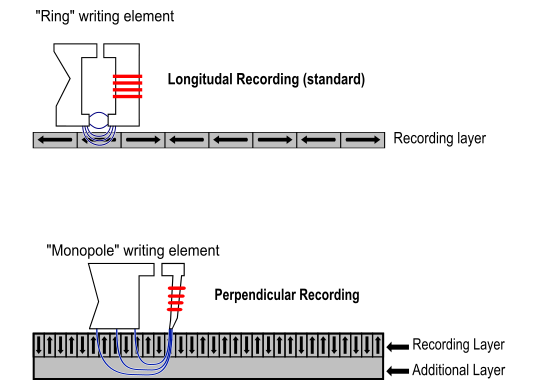
\includegraphics[scale=.45]{perpendicularComparison.png}}
\caption{Perpendicular recording due to the presence of the additional layer, soft underlayer, a much larger magnetic field can be applied to the recording layer. This allows us to use material with higher anisotropy meaning the domain size can be reduced and density increased.}
\label{perpendicularComparison}
\end{figure}


However, this too will have a limit at a smaller domain size where thermal fluctuations will be an issue again. One method still currently in development is called heat-assisted magnetic recording (HAMR). This method is based on the fact that all ferromagnetic materials have a curie temperature where the internal magnetic field the material had is lost and aligns itself to any external magnetic field. In HAMR, when a bit needs to get written to, a laser is used to heat up the desired domain to the curie temperature allowing the magnetic field generated by the write head to align the domain, and then allowing the material to cool back down. This means that the recording material can be changed to one with a much higher anisotropy value allowing the domain sizes to decrease even more, further increasing the storage density to around 1TB/in$^2$ \cite{hamr}. 



\section{Flash Memory}
Flash memory is has been becoming more and more popular recently as a replacement for hard drives due to their speed. They are already commonly used in flash drives but are becoming more and more popular. One of the most, if not the most, important device in flash memory and modern computing and as a whole is the transistor. A transistor is able take in a circuit input and act as a switch turning another circuits on or off without any moving parts. This ability to switch off and on a circuit will prove crucial in saving bits of memory.

\subsection{Semiconductors}
To explain how transistors work, first we need to explain what a semiconductor is since a transistor is a semiconductor device. A bandgap diagram is useful in describing semiconductors. Band structure represents the specific energy levels that electrons can occupy due to quantum mechanics. However, only the valence band and the conduction band are relevant when discussing conductivity. The valence band is the highest energy levels that electrons can occupy at absolute zero temperature while the conduction band is where electrons can move freely. As seen in Fig. \ref{bandGap}, the conductor is any material that doesn't have a bandgap between the valence band and conduction band meaning all the electrons can move freely. An insulator is any material whose conduction band is separated by a large band gap from its valence band. This means that the valence electrons can not easily move to its conduction band and thus are not free too move. Lastly, a semiconductor is any material whose conduction band is separated from the valence band by a band gap small enough that thermal fluctuations can excite electrons to the conduction band \cite{purcell}.


\begin{figure}[H]
\centerline{\includegraphics[scale=.45]{bandGap.png}}
\caption{a) Metals/conductors are materials which have their valence electrons are free to move in the overlapping conduction band. Insulators, c, are materials which have their valence electrons are unable to move in their valence band and is unable to easily access the conduction band. Semiconductors, b, are materials which have their electrons unable to move in their valence band, but is easily exicted into the conduction band where they can carry current.}
\label{bandGap}
\end{figure}


Most commercial applications of semiconductors use impurity semiconductors. Impurity semiconductors are materials that gain different properties than pure semiconductors by adding an impurity, dopant, to the material. For example, say we have silicon with 4 valence electrons where each valence electron is shared with another silicon atom to create tetrahedron. Then if we replace one of those silicon atoms with a phosphorus atom with 5 valence electrons, 4 of the 5 valence electrons will be shared with the 4 nearby silicon atoms, but the last one is loosly bound to the phosphorus. At room temperature, thermal energy is enough to release it from this loosly bound state and it becomes a conduction electron. This is called n-type doping. If instead of adding an element with 5 valence electrons and instead added one with only 3, we would then have one less electron than its pure state which is represented as a hole.This is called p-type doping \cite{purcell}.

A simple example of a semiconductor device is the pn junction diode. This device is created when a p-type semiconductor is comes in contact with an n-type semiconductor. Since p-type materials have a higher concentration of holes than the n-type, holes diffuse across to the n-type material while electrons diffuse the other way; this is the diffusion current. The holes and electrons that diffuse then recombine in the n-type and p-type material respectively. This creates a depeltion zone at the intersection of the two materials. The diffusion and recombination also creates a net positive charge on in the p-type material and a net negative charge in the p type material creating an Electric field towards the p-type. The diode is in equilibrium when the drift current and diffusion current are equal.


\begin{figure}[H]
\centerline{\includegraphics[scale=.7]{pnJunction.png}}
\caption{This is a diagram of a pn junction diode with current in different directions. In the clockwise current in a, the holes and electrons are constantly refreshed due to the applied potential, and the current can continuously flow. In the counterclockwise current, b, the applied potential increases the depeletion zone until the local electric field cancels out the applied potential and stops the flow of current.}
\label{pnJunction}
\end{figure}

The special property of a PN junction is that current is only allowed to flow in one direction. Fig. \ref{pnJunction} shows what happens when a clockwise current is applied and when a counterclockwise current is applied. In Fig. \ref{pnJunction}a, the clockwise current pushes holes from the p type and electrons from the n type towards the interface where they combine and produce heat. So the diode loses electrons and holes at the interface due to recombination, however the current pulls electrons from the p type resupplying the p type with holes. The converse happens in the n type so a current can flow indefinitely. This is known as forward bias. In Fig. \ref{pnJunction}b the counter-clockwise current directs the holes in the p type and the electrons in the n type flow away from the interface. The flow of electrons and holes away from the interface continues until the local electric field produced is strong enough to oppose the applied potential, causing the current to stop; this is known as reverse bias \cite{thermo} 




\subsection{Transistors}
So now that we know what p-type and n-type doped semiconductors and pn junction diodes are, we can now talk about transistors. While there are many different types of semi conductors, the one that flash memory uses is the metal oxide semiconductor field effect transistor (MOSFET). A MOSFET, as seen in Fig. \ref{mosfet}a consists of a p-type silicon with two n-type regions, one on each side as a source and drain, and a metal gate separated from the semiconductor by an insulating oxide layer (typically SiO$_2$) in the middle. When no voltage is applied to the gate as seen in a, the MOSFET acts as two pn diodes, and so any voltage difference between the source and drain will reverse bias one of the two pn diodes so no current will flow. However, if a positive voltage is applied to the gate, the positive charge attracts electrons and repels holes as in Fig. \ref{mosfet}b. If the voltage applied to the gate is above a certain threshold of around 1V, a thin layer of electrons will be formed under the oxide. Also known as the inversion layer, this creates a conducting channel between the source and drain, and the p-type silicon acts as an n-type material at the oxide layer due to the extra electrons allowing current to flow between the source and drain. This change created by the field from the gate is why it is called a field effect transistor. One advantage MOSFETS have over other transistors is that the MOSFET requires nearly no current, so the input power is much less and there will be less issues with self-heating, which can be an issue since they're so tightly packed together\cite{modernPhysics}.


\begin{figure}[H]
\centerline{\includegraphics[scale=.45]{mosfet.png}}
\caption{ a) is a normal MOSFET without any applied charge and thus acts an npn semiconductor and doesn't let current flow. b) The positive charge on the metal gate cause electrons to build up along the oxide layer/semiconductor interface between the two n drops. This causes the semiconductor to turn into a n type semiconductor which allows current to flow.}
\label{mosfet}
\end{figure}

What is actually used to store bits is called the floating gate transistor. It is the same as the MOSFET except instead of only having one gate above the insulating oxide, you have another layer of insulating oxide on the other side of the gate followed by another gate called the control gate. So now the middle gate, also known as the floating gate, is electrically isolated due to the oxide layer on each side. Because of this, the only way to add and remove charge is through Fowler-Nordheim tunneling.  This means that when positive charge is stored on this gate, current will pass through and send a 1 and a 0 otherwise. Since the charges on the floating gate can not leave it without tunneling, that means that even when the transistor isn't powered, it will still store its memory. 

One method used to increase storage density is to change from using single level cells (SLC) to multi level cells (MLC) and three level cells (TCL). SLC is the standard floating gate where it either outputs a 1 or 0 by dividing the gate into two possible states, current or no current. However, the MLC stores 2 bits instead of one by dividing the gate into 4 possible states. While this has the benefit of doubling the storage density, it allows more room for error since the states are smaller and more difficult to distinguish. The oxide layer that was being used previously degraded after certain number of uses, and this degradation would become more visible on MLC drives first because they have to be able to disntinguish states more than SLC. However, advancements in both the oxide layer and also dynamic mapping of memory such that no one gate is used more than the other means that this have become less of an issue.

\section{Future Technology}

While these three types of storage already exist for the most part, we need to look into other techniques to store data as the world creates more and more of it. Two possible techniques are holographic data storage and probe based storage.
\subsection{Holographic Data Storage}
Holographic data storage (HDS) has the potential to store over 1Tb/in$^2$. In the most basic sense, holography is the method of capturing and recreating optical information through interference patterns, and a hologram is a recording of an interference pattern. Fig. \ref{create} shows how to record a hologram; first a coherent light source is split into a reference and object beam using a beam splitter. The object beam is reflected off the object being recorded on to the photographic plate. The reference beam, also being shone on to the photographic plate,  interferences with the object beam and that interference pattern is recorded on the plate as a hologram. Destructive interference appears as dark spots and constructive interference appears as bright spots. 

\begin{figure}[H]
\centerline{\includegraphics[scale=.45]{create.png}}
\caption{This is an example of a transmission hologram where a coherent souce of light is split into a reference beam and an object beam. The two beams eventually create an interference pattern at the photographic plate creating a hologram \cite{HDS}.}
\label{create}
\end{figure} 

 To recreate the image from the hologram, the reference beam in Fig. \ref{reconstruct} is shone back at the hologram at the same angle and by looking at where the object should be through the hologram, a virtual image can be seen of the object. This is due to the reversibility of light which states that light will take the same path if the direction it travels is reversed. So when we shine the reference beam through the hologram and view it with our eyes, our eyes trace the light back the same path it took when the hologram was created with the object beam and see a virtual image.

\begin{figure}[H]
\centerline{\includegraphics[scale=.45]{reconstruct.png}}
\caption{To recreate the virtual image, the reference beam is shined on the hologram at the same angle, and by looking through the hologram to where the object should be, a virtual image can be seen \cite{HDS}.}
\label{reconstruct}
\end{figure} 

Another way to look at this would be quantitatively. First, the reference beam can then be represented a complex electric field,

\begin{equation}
E_{R} = re^{i(\omega t + \phi)},
\label{eRef}
\end{equation}

where r is the amplitude of the beam and is assummed to be constant over the surface of the film due to the plane wavefront of the reference beam (wavefront is the collection of points that have the same phase and thus same amplitude) \cite{optics}. $\omega$ is simply the angular frequency, and $\phi$ is the phase angle that relates to the tilt of the photographic plate relative to the reference beam and can be described by

\begin{equation}
\phi = (\frac{2\pi}{\lambda})\Delta = (\frac{2\pi}{\lambda})x sin \alpha
\label{phi}
\end{equation}

when the top border of the beam hits the plate at x = 0. As seen in Fig. \ref{eRefMath},$\delta$ is the extra distance traveled by certain parts of the wavefront depending on the angle of the beam relative to the normal, $\alpha$.

\begin{figure}[H]
\centerline{\includegraphics[scale = .12]{eRefMath.jpg}}
\caption{The intersection of the reference beam and the photographic film \cite{optics}.}
\label{eRefMath}
\end{figure} 

 Similary, the subject beam can be represented by,
\begin{equation}
E_{S} = re^{i(\omega t + \theta)},
\label{eSub}
\end{equation}
where s is the ampltiude of the reflected light off the object, and $\theta$ is analogous to $\phi$ except that it is more complicated due to variations in the phase of the light because it is reflected from different parts of the object \cite{optics}. 

The resultant electric field at the plate is then given by
\begin{equation}
E_{P} = E_R + E_S.
\label{Ef}
\end{equation}

The quantitiy that describes the hologram is known as scaled irradiance which is defined as the magnitude squared of the electric field. Thus, the scaled irradiance at the plate, is given by
\begin{equation}
I_{P} =  |E_P|^2 = (E_R + E_S) (E^*_{R} + E^*_{S}).
\label{If}
\end{equation}

By multiplying the binomials and subbing in for $E_R$ and $E_S$ from Equations \ref{eRef} and \ref{eSub}, respectively, $I_P$ can be simplified to \cite{optics}
\begin{align}
\begin{split}
I_{P} &= r^2 + s^2 + E_S E^*_R + E_R E^*_S  \\
I_{P} &= r^2 + s^2 + rse^{i(\theta - \phi)} + rse^{-i(\theta - \phi)}.
\end{split}
\label{IfFinal}
\end{align}

Then by shining the reference beam back through the hologram, we can recreate the image of the object. This can be expressed as
\begin{equation}
E_H =  I_F E_R = (r^2 +s ^2)E_R + r^2se^{i(\omega +\theta)} + r^2e^{i(2\phi)}e^{i(\omega t-\theta)}.
\label{Eh}
\end{equation}

The first term of $E_H$ represents the reference beam that has been amplitude-modulated but not phase-modulated, so it passes straight through the hologram. The second term represents the subject beam that has been amplitude-modulated by a factor of $r^2$. This term represents the reconstructed wavefront from the subjectand strikes the plate at an angle $\alpha$. This is the virtual image seen typically viewed and is a virtual image since no light is present at the image, rather it is created due to our eye reversing the light back to the image. The last term represents the an amplitude and phase-modulated subject beam. Since it is phase modulated as well, it appears on the opposite side of the hologram and is a real image. 

Moving on, holograms can be created in both thick and thin regimes. The thin regime is unsuitable for high density storage because thin holograms like those written on photographic film confine their diffractive interaction to a single plane and can't be used for multiplexing \cite{HDS}. The criterea used quantify the thickness or thinness of a hologram is known as the $Q$ parameter. The $Q$ parameter is given by 
\begin{equation}
Q = \frac{2\pi\lambda L}{n_0\Lambda^2},
\label{qParameter}
\end{equation}
where $\lambda$ is the wavelength of the light, $L$ is the thickness of the recording layer, $n_0$ is the index of refraction of the medium, and $\Lambda$ is the grating period. A hologram is considered in the thin regine if $Q<1$ and is considered in the thick regime if $Q>1$. The thickness of the medium can range from 500$\mu$m to a few millimeters \cite{HDS}.

To store digital data in holograms, a spatial light modulator (SLM) is needed. The SLM converts the 1s and 0s of the digital data into light and dark pixels respectively onto a 2D image called a page. The number of bits that can be stored per SLM image can be over one million, but this varys with the SLM's pixel count. So to record digital data, instead of reflecting the object beam off of the object, it is shone through the SLM then onto the storage medium as seen in Fig. \ref{dataHologramCreate}. 

\begin{figure}[H]
\centerline{\includegraphics[scale=.45]{dataHologramCreate.png}}
\caption{This implementation of holographic storage uses the same technique as a transmission hologram except instead of reflecting the object beam off of the object, it is shone through the SLM which contains the bit information. Since the SLM page contains many bits at once, it can write more than one bit at once unlike magnetic drives.}
\label{dataHologramCreate}
\end{figure} 
Reading the hologram is the same as it would be for a thin hologram. The reference beam is shone at the hologram, but now there is a detector array to convert the SLM image of dark and bright spots into 1s and 0s for the computer. Since a page of bits can be read/written all at once instead of bit by bit, HDS has the ability to have much greater read write speeds over other competing technologies such as magnetic data storage.
\begin{figure}[H]
\centerline{\includegraphics[scale=.45]{dataHologramReconstruct.png}}
\caption{Reading information is the same as recreating a hologram except now the virtual image is shone onto a detector array which converts the dark and bright spots into 1s and 0s.}
\label{dataHologramReconstruct}
\end{figure} 
The reason why HDS can be so dense is because of its ability to superimpose holograms in the same volume; this is known as multiplexing. HDS offers many different methods for multiplexing. An important parameter in multiplexing is called the diffraction efficiency, $\eta$, which is the ratio of the diffracted optical power divided by the incident optical power and is expressed as 
\begin{equation}
\eta = sin^2(\sqrt{\nu ^2 + \xi ^2})/(1 + \frac{\xi ^2}{\nu ^2})
\label{dE}
\end{equation}
where $\nu$ and $\xi$ are defined as 
\begin{equation}
\nu = \frac{\pi n_1L}{\lambda(cos^2\theta - \frac{Kcos\phi}{\beta})^{1/2}}
\label{nu}
\end{equation}
and
\begin{equation}
\xi = \frac{[\Delta\theta K sin(\phi - \theta_o) - \Delta\lambda K^2 / 4\pi n_0]d}{2(cos\theta - \frac{Kcos\phi}{\beta})}.
\label{xi}
\end{equation}

In above equations are for a pure index grating in a transmission hologram where $n_1$ is the index perturbation, $L$ is the thickness of the recording layer, $\theta$ is the angle of the reference beam outside the media, $K$ is the grating number, $n_o$ is the bulk index of the material, $\phi$ is the grating slant angle inside the material, $\beta$ is $2\pi (epsilon_o)^(1/2)/\lambda$, where $epsilon_o$ is the bulk dielectric constant, $\Delta \Lambda$ is the discrepancy from the Bragg condition (constructive interference from reflection off of grating) for wavelength, and $\Delta \theta$ is the discrepancy from the Bragg condition for angle. A diffraction efficiency of 0% would mean that the diffracted portion would have completely destructively interfered.

One category of methods is known as Bragg-Based techniques which rely on the Bragg effect/condition. Since the angle of the reference beam must match exactly the angle it had when recording the hologram, that means that a small change in the angle when recreating the image will cause the image to not appear sharply or at all. We can use this sensitivity by having one page of data from the SLM stored at one angle and another page in the same volume by changing the angle of of entry. More specifically, the spacing between the diffraction max and the first null in the diffraction efficiency, angular selectivity, is given by
\begin{equation}
\Delta \theta = \frac{\lambda cost\theta_s}{Lsin(\theta_r + \theta_s)},
\label{angular}
\end{equation}
where $\theta_r$ and $\theta_s$ are the reference and signal(object) angles and $L$ is the media thickness. To minimize noise and interference between different pages, each page would have its Bragg peak at the null position in the diffraction efficiency of every other page by changing the reference angle in by multiples of the angular selectivity. A similar method to add multiplexing is to vary the wavelength of the the source and reference beams. This method is limited due to the small tuning range of lasers. Yet another method is to vary the point of entry of the beams into the medium. While there are more methods of multiplexing, the true benefit of multiplexing occurs when combining multiple multiplexing techniques at once. For example, hybrid wavelength and angular multiplexing systems have been tested before \cite{memory}. 

\section{Conclusion}
Digital data storage allows us to store our digital information in a variety of different methods. We're already able to store data at incredible densities or speeds, but as more and more information is being saved digitally we will need more and more dense and efficient ways to store our data. Since only two states are needed to store memory, it is very easy to find techniques to store memory like punch cards. However, it is quite difficult to find technique that are dense and efficient. As we've seen, there is continued improvements being made to current data storage techniques such as Blu-Ray discs and the change to perpendicular recording in hard drives. However, these are only short term solutions to our storage needs. Both holographic storage and probe storage are new techniques that each have the potential to store over 1 Tb/in$^2$, but they each have their own issues that currently keep them in the development stage. As our data needs keep growing, the technology needed to support that will continue to evolve as well.



\bibliographystyle{aip}
\bibliography{myCollection2}



\end{document}
